% \chapter{Beispielhafte Integration}
	
\section{Anforderungen}
%\section{Anforderungen}
%\textit{Hier soll definiert werden, welche Kriterien der PoC erfüllen soll und wenn möglich sollen zusätzlich Möglichkeiten zur Überprüfung dieser Kriterien definiert werden.}

Das zu erstellende Proof-of-Concept soll einige Rahmenbedingungen erfüllen. In diesem Abschnitt werden diese Bedingungen näher beschrieben.
	
\subsection{Definitionen}
	
Um die Anforderungen systematisch einzuordnen, werden folgend zwei Modelle vorgestellt, anhand dessen die Kategorisierung erfolgt.

Beim ersten Modell handelt es sich um das Kano-Modell \cite{KanoModell} der Kundenzufriedenheit, welches in  \autoref{tab:merkmale-nach-dem-kano-modell} erläutert wird.
	
\begin{table}[H]
\begin{tabular}{ |p{1.15cm}|p{2.75cm}|p{9.6cm}| }
	\hline
	Kürzel & Titel & Beschreibung \\
	\hline
	\textbf{B} & Basis\-merkmal & Merkmale, die als selbstverständlich angesehen werden. Eine Erfüllung erhöht kaum die Zufriedenheit, jedoch eine Nichterfüllung führt zu starker Unzufriedenheit \\
	\hline
	\textbf{L} & Leistungs\-merkmal & Merkmale, die der Kunde erwartet und bei nicht Vorhandensein in Unzufriedenheit äußert. Ein Vorhandensein erzeugt Zufriedenheit, beim Übertreffen umso mehr. \\
	\hline
	\textbf{S} & Begeisterungs\-merkmal & Merkmale, die eine Herabsetzung von der Konkurrenz ermöglichen und die den Nutzenfaktor steigern. Sind sie vorhanden, steigern sie die Zufriedenheit merklich. \\
	\hline
	\textbf{U} & Unerhebliches Merkmal & Für den Kunden belanglos, ob vorhanden oder nicht. \\
	\hline
	\textbf{R} & Rückweisungs\-merkmal & Diese Merkmale führen bei Vorhandensein zu Unzufriedenheit, sind jedoch beim Fehlen unerheblich. \\
	\hline
\end{tabular}
 \captionsetup{justification=centering}
  \caption{Merkmale nach dem Kano-Modell der Kundenzufriedenheit}
   \label{tab:merkmale-nach-dem-kano-modell}
\end{table}

Neben der Unterscheidung nach dem Kano-Modell werden die Anforderungen in funktionale und nicht-funktionale Anforderungen \cite{FunktionaleUndNichtFunktionaleAnforderungen} aufgeteilt (vgl. \autoref{tab:kategorien-der-anforderungsliste}).

\begin{table}[H]
\begin{tabular}{ |p{1.15cm}|p{2.75cm}|p{9.6cm}| }
	\hline
	Kürzel & Titel & Beschreibung \\
	\hline
	f & funktional & Beschreiben Anforderungen, welche ein Produkt ausmachen und von anderen differenzieren (\enquote{Was soll das Produkt können?}). Sie sind sehr spezifisch für das jeweilige Produkt. Ein Beispiel: Das Frontend fragt Daten für X vom Partnersystem 1 über eine SOAP-API ab, etc.\\
	\hline
	nf & nicht-funktional & Beschreiben Leistungs- und Qualitätsanforderungen und Randbedingungen (\enquote{Wie soll das Produkt sich verhalten?}). Sie sind meist unspezifisch und in gleicher Form auch in unterschiedlichsten Produkten vorzufinden. Beispiele sind: Benutzbarkeit, Verfügbarkeit, Antwortzeit, etc. Zur Überprüfung sind oftmals messbare, vergleichbare und reproduzierbare Definitionen notwendig. \\
	\hline
\end{tabular}
 \captionsetup{justification=centering}
  \caption{Kategorien der Anforderungen}
   \label{tab:kategorien-der-anforderungsliste}
\end{table}
	
\subsection{Anforderungsanalyse}

Die Anforderungen, welche von der zu erstellende Lösung gefordert werden, ergaben sich durch den Einfluss verschiedener Quellen. Die primäre Quelle an Anforderungen stellen die Stakeholder dieser Arbeit, Christian Wansart und Stephan Müller, dar. Als Stakeholder betreuen sie die Arbeit und haben ein eigenes Interesse, dass aus der Arbeit ein erfolgreiches und übertragbares Ergebnis resultiert.

Neben den Stakeholdern ergeben sich auch Anforderungen direkt aus der Forschungsfrage selbst und den Bestrebungen des Autors. Die Quellen werden in den Anforderungen mit einem Kürzel angegeben, wie z. B. \texttt{A} für Autor, zu sehen in \autoref{tab:quellen-der-anforderungen}.

Eine dritte Quelle von Anforderungen ergibt sich aus der Problemstellung des Kunden der Open Knowledge, welche in der Motivation angesprochen wurde. Die beiden Stakeholder brachten neben ihren eigenen Bestrebungen auch die Rahmenbedinungen und Wünsche des Kunden mit ein. Aus dieser Kommunikation ergaben sich somit weitere Anforderungen, welche einen realitätsnahen Charakter haben.

Anforderungen können auch eine Kombination von mehreren Quellen besitzen, wenn die Anforderung aus einer gemeinsamen Bestrebung oder Diskussion entstand.

\begin{table}[H]
\begin{tabular}{ |p{1.15cm}|p{1.9cm}|p{10.45cm}| }
	\hline
	Kürzel & Titel & Beschreibung \\
	\hline
	A & Autor & Hiermit ist der Autor dieser Arbeit gemeint. \\
	\hline
	S & Stakeholder & Die beiden Stakeholder Christian Wansart und Stephan Müller \\
	\hline
	K & Kunde & Ein Kunde der Open Knowledge, ein Direktversicherer. \\
	\hline
\end{tabular}
 \captionsetup{justification=centering}
  \caption{Quellen der Anforderungen}
   \label{tab:quellen-der-anforderungen}
\end{table}
	
\subsection{Anforderungsliste}

Um die Anforderungen strukturiert zu erfassen, werden sie ähnlich einer Karteikarte, wie in \autoref{tab:beispiel-anforderung} zu sehen, dargestellt. Hierbei erhält jede Anforderung eine Kategorisierung nach dem Kano-Modell, ob sie funktional oder nicht-funktional ist und aus welcher Anforderungsquelle sie entstammt. Jede Anforderung erhält zudem eine eindeutige Id, die nachfolgend in der Arbeit zur Referenzierung dient.

\begin{table}[H]
\begin{tabular}{ |p{1.25cm}|p{5.5cm}|p{2.25cm}|p{2.1cm}|p{1.25cm}| }
\hline
Id            & Name          & Kano-Modell   & Funktionsart  & Quelle        \\
\textit{1234} & \textit{Dummy} & \textit{S} & \textit{nf} & \textit{S} \\
\hline
\multicolumn{5}{|l|}{\textit{Hier wird die Anforderung beschrieben.}} \\
\hline
\end{tabular}
 \captionsetup{justification=centering}
  \caption{Beispiel einer Anforderung}
   \label{tab:beispiel-anforderung}
\end{table}

% use generated list

% textidote: ignore begin

\subsubsection{Grundanforderungen}


\subsubsection{Funktionsumfang}


\begin{anf}{anf:1010}{1010}{Schnittstellen-Logging}{B}{f}{S}
\multicolumn{5}{|p{14.05cm}|}{Das Aufrufen von Schnittstellen soll mittels einer Logmeldung notiert werden. Hierbei sollen relevante Informationen wie Aufrufparameter mit notiert werden.} \\
\hline
\end{anf}

\begin{anf}{anf:1011}{1011}{Use-Case-Logging}{B}{f}{S}
\multicolumn{5}{|p{14.05cm}|}{Tritt ein Use-Case auf, soll dieser im Log notiert werden. Beispielsweise soll notiert werden, dass ein Nutzer einen neuen Datensatz angelegt möchte und wenn der diesen anlegt.} \\
\hline
\end{anf}

\begin{anf}{anf:1100}{1100}{Logübertragung}{B}{f}{S}
\multicolumn{5}{|p{14.05cm}|}{Ausgewählte Logmeldungen sollen an ein Partnersystem weitergeleitet werden. Die Auswahl könnte über die Kritikalität, also dem Log-Level, der Logmeldung erfolgen.} \\
\hline
\end{anf}

\subsubsection{Eigenschaften}


\begin{anf}{anf:2010}{2010}{Resilienz der Übertragung}{S}{f}{S}
\multicolumn{5}{|p{14.05cm}|}{Daten die der Nachvollziehbarkeit dienen, sollen wenn möglich bei einer fehlgeschlagenen Verbindung nicht verworfen werden. Sie sollen mindestens 120s vorgehalten werden und in dieser Zeit sollen wiederholt Verbindungsversuche unternommen werden.} \\
\hline
\end{anf}

\begin{anf}{anf:2020}{2020}{Batchverarbeitung}{S}{f}{S}
\multicolumn{5}{|p{14.05cm}|}{Daten, die der Nachvollziehbarkeit dienen, sollen wenn möglich gruppiert an externe Systeme gesendet werden. Hierbei ist eine kurze Aggregationszeit von bis zu 10s akzeptabel.} \\
\hline
\end{anf}

\subsubsection{Partnersysteme}

% textidote: ignore end
	
\section{Vorstellung der Demoanwendung}

	\textit{In diesem Abschnitt soll die Demoanwendung vorgestellt werden, anhand dessen das Proof-of-Concept erstellt wird. Damit das Proof-of-Concept erstellt werden kann, muss die Demoanwendung die zuvor beschriebenen Probleme aufweisen, hierbei sollen die Probleme möglichst realitätsnah sein und nicht frei erfunden.}
	
\newpage
	
\section{Konzept}
	
	\subsection{Datenverarbeitung}

	Auf Basis der zuvor vorgestellten Methoden und Praktiken wird nun eine sinnvolle Kombination konzeptioniert, die als Ziel hat, die Nachvollziehbarkeit nachhaltig zu erhöhen. Es werden die Disziplinen Datenerhebung, -auswertung und -visualisierung unterschieden und nacheinander beschrieben. Danach und darauf aufbauend wird eine grobe Architektur vorgestellt, die diese Ansätze in ein Gesamtbild bringt.
		
	\subsubsection{Erhebung}
		
	Im Standardfall erhalten Betreiber und Entwickler, bis auf die Kommunikation mit Partnersystemen, keine Informationen von einer SPA. Deswegen sollen zunächst Loginformationen des Frontends erhoben und an ein weiteres System gesendet werden. Hierbei ist eine Unterscheidung sinnvoll, welche Logmeldungen tatsächlich gesendet werden sollen (bspw. anhand des Log Kritikalität). Diese Unterscheidung sollte konfigurativ änderbar sein. Dieser Datenstrom wird erfahrungsgemäß unregelmäßig aber doch schon sehr häufig mit Daten befüllt, um eine gute Nachvollziehbarkeit zu erreichen.
		
	Neben den Loginformationen sollten nicht gefangene Fehler und optional gefangene Fehler an ein weiteres System weitergeleitet werden. Dabei sollen alle relevanten und zugreifbaren Informationen mitgesendet werden.
		
	Eine Datenerhebung wie beim Real-User-Monitoring, wo jede Benutzerinteraktion aufgezeichnet wird um bspw. Klickpfade zu optimieren um festzustellen wie lange sich Nutzer auf einer Seite aufhalten. Jedoch ist ein Session-Replay Mechanismus enorm hilfreich und gewünscht, welcher ebenso jede Benutzerinteraktion aufzeichnen muss. Damit nicht zu viele Daten erhoben werden und damit nicht jede Nutzersitzung mitgeschnitten wird, soll die Aufzeichnung erst nach Einwilligung und Aktivierung Seitens des Nutzers erfolgen oder bei speziellen Umgebungen automatisch (bspw. eine Staging-Umgebung). Weiterhin könnten die Loginformationen nach dieser Einwilligung auch feingranularer übertragen werden, bspw. ohne Einwilligung würden Logs der Kritikalität INFO und höher übertragen werden und mit Einwilligung auch Logs der Kritikalität DEBUG und höher.
		
	Des Weiteren soll ein Tracing der Kommunikation zwischen Frontend und Partnersystemen eingesetzt werden. Bei könnten wichtige Verarbeitungsmethoden auch im Tracing erfasst werden, dies wird jedoch hier nicht definiert und ist Teil der eigentlichen Implementierung. Es soll wenn möglich auf den neuen Standard OpenTelemetry (OTel) aufgesetzt werden. Hierdurch wird das Erheben von Tracing- und Metrikdaten standardisiert und zukünftig auch bei Logdaten. Auf Basis von OTel sollen beispielhaft Metriken erfasst werden, um das Anwendungsverhalten nachzuhalten und zu überwachen. Durch diese Metriken können Aspekte eines Application Performance Monitorings erfüllt werden.
		
	Alle gesendeten Datensätze sollen möglichst mit Metadaten angereichert werden, die einerseits den Nutzer, die Umgebung und die Anwendung identifizieren. Diese umfassen u. A.: Zeitstempel, Session-Id, User-Agent, IP, Hostsystem, Version.
		
	\subsubsection{Auswertung}
		
	Bei der Auswertung der Daten soll hauptsächlich auf bestehende Technologien gesetzt werden, wie z.B. die Technologien, die in \autoref{sec:werkzeuge-und-technologien} evaluiert wurden. Das heißt im Konzept kann nicht im Detail darauf eingegangen werden, wie diese Daten tatsächlich verarbeitet werden und ist auch nicht direkt von Relevanz. Eine Beschreibung folgt im \autoref{sec:technologie-stack} sowie beim Einsatz von den Technologien selbst.
		
	Lediglich bei der Vorverarbeitung des Tracings im Client kann nun bereits eine Aussage getroffen werden. Wird hierbei nämlich, wie gewünscht, auf OTel gesetzt, dann erfolgt eine Vorverarbeitung von den Komponenten von OTel selbst. Dabei werden die u. A. Spankontexte fürs Tracing und die Beziehung zwischen den Spans gepflegt.
		
	\subsubsection{Visualisierung}
		
	Wie bei der Auswertung wird auch die Visualisierung stark abhängig von den eingesetzten Technologien sein. Nichtsdestotrotz können bereits hier gewünschte Ansichten/Funktionen definiert werden:
		
	\begin{itemize}
		\item Die Logdaten sollen abrufbar sein und filterbar sein.
		\item Fehlerinformationen sollen gesondert der Logdaten dargestellt werden.
		\begin{itemize}
			\item Fehler sollen gruppiert werden, um gleiche Fehlerbilder zusammenzufassen.
			\item Zu den Fehlerbildern sollen übergreifende Informationen dargestellt werden.
			\item Es lassen sich auch einzelne Fehler einer Fehlergruppe anzeigen.
		\end{itemize}
		\item Für einen ausgewählten Trace soll ein Trace-Wasserfallgraph dargestellt werden (vgl. \autoref{sec:tracing})
		\item Die beispielhaften Metriken soll visuell dargestellt werden.
		\item Die Daten zum Session-Replay sollen, wenn vorhanden, visuell dargestellt werden, sodass die Interaktionen des Nutzers nachzuvollziehen sind.
	\end{itemize}
	
	\subsection{Architektur}

	Auf Basis der zuvor definierten Grundkonzepte zur Datenverarbeitung, wird nun eine grobe Architektur konzipiert. Im Allgemeinen sollen die Funktionsbereiche Log Management, Error Monitoring, Application Monitoring, Tracing sowie Session-Replay erfüllt werden. Im Client soll es für jeden Funktionsbereich eine eigene Komponente geben, die die jeweiligen Daten erfasst und an das entsprechende Partnersystem weiterleitet. Lediglich die Erfassung von Metriken und Tracing soll auf Basis von OpenTelemetry erfolgen und daher dieselben Komponente verwenden. Dieser Aufbau lässt sich auf der linken Seite der \autoref{fig:grobe-architektur} betrachten.
	
	Für die Datenverarbeitung, -analyse und -visualisierung von Logs, Fehlern und Metriken soll eine einzelnes System zuständig sein. Denn für die Bewältigung dieser verschiedenen Kategorien sind ähnliche Disziplinen notwendig, wodurch ein einzelnes System ausreichen sollte. Grundlegende Funktionen dieses Systems belaufen sich auf die Langzeitspeicherung, eine performante Suche und die Visualisierung in Graphen.
	
	Für Tracing wird ein zweites System benötigt, hauptsächlich weil in der Evaluation kein Werkzeug identifiziert werden konnte, welches neben den zuvor genannten 3 Datenkategorien auch Tracingdaten gut unterstützt. Tracingdaten sind zudem anders, dadurch dass sie einen hohen Datendurchsatz aufweisen und zudem eine große Menge darstellen.
	
	Ein drittes System soll die Funktionalität rund um Session-Replay übernehmen. Hierbei liegt auch der Grund darin, dass kein Werkzeug identifiziert werden konnte, welches neben Session-Replay auch andere Disziplinen erfüllen kann. Weiterhin sind, wie beim Tracing, die Eigenschaften der Daten anders, denn hier werden nahezu konstant Daten versendet, um alle Benutzerinteraktionen und das Anwendungsverhalten nachstellen zu können.
	
\begin{figure}[H]
	\centering
	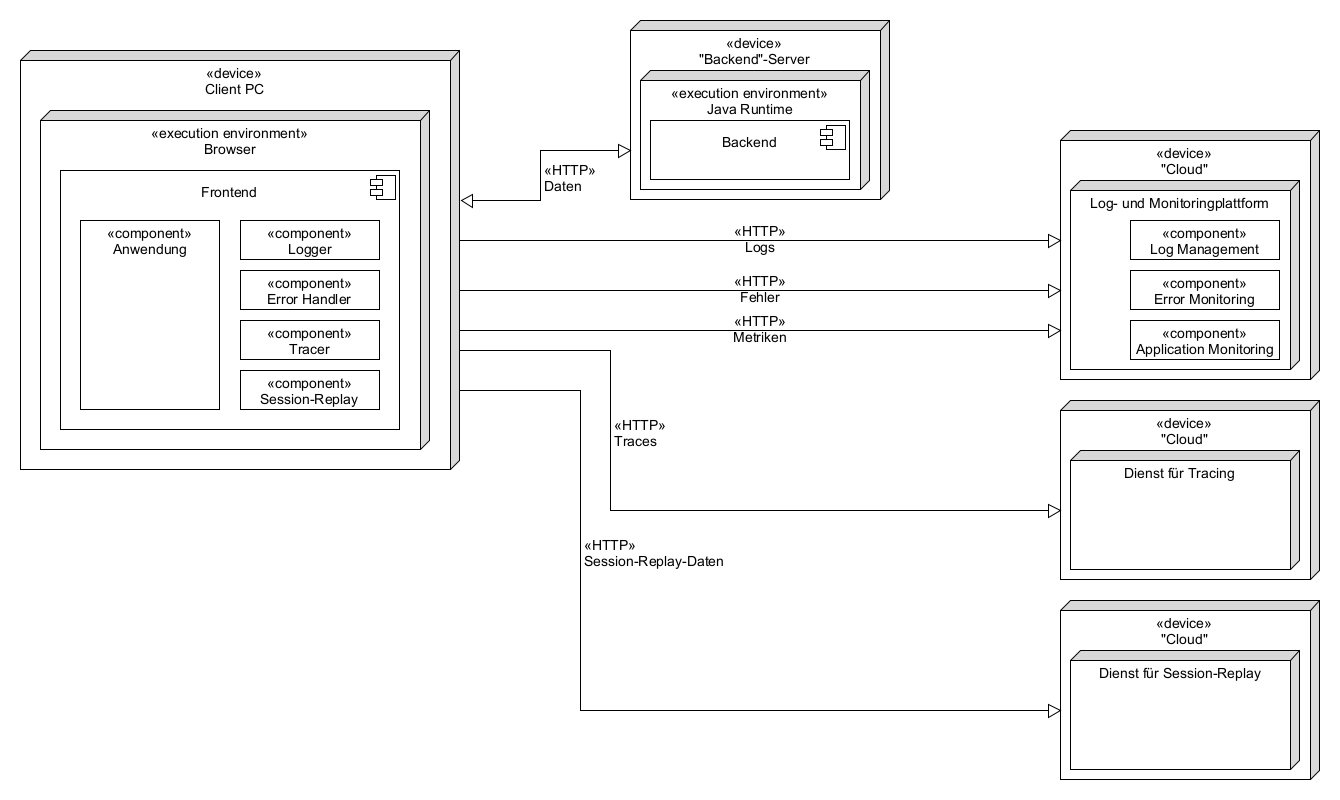
\includegraphics[width=0.75\linewidth]{img/04_erstellung-poc/konzept-simple.png}
	\caption{Grobe Architektur}
	\label{fig:grobe-architektur}
\end{figure}

Wie in der Datenerfassung erwähnt, werden die einzelnen Datentypen unterschiedlich erhoben und besitzen somit auch eine andere Eigenschaften. Wie IBM bei Big Data definiert \cite{ZikopoulosUnderstandingBigData}, lassen sich auch hier die Eigenschaften Volume, Velocity und Variety identifizieren. Der Aspekt Volume ist weniger präsent, denn die Datenmengen sind nicht vergleichbar mit echten Big-Data-Anwendungen. Genau ist dies nicht prognostizierbar, aber in der Evaluierung des Stands der Technik, ließ sich ein Datendurchsatz von 1 MB/min feststellen - somit stellt dies im Frontend keine Herausforderung dar, jedoch in den verarbeitenden Systemen kann dies natürlich durch eine große Menge an Frontends multipliziert werden, was jedoch nicht im Fokus der Arbeit steht.

Eine Variety der Daten, also Unterschiedlichkeit der Datenstruktur, ist definitiv vorhanden und entspringt den verschiedenen Funktionsgebieten. Auch innerhalb derselben Datenströme kann eine Variety identifiziert werden, denn bspw. sind Logmeldungen sehr individuell, sie folgen meist nicht streng einem Format und enthalten unterschiedliche Menge an Informationen.

Der Aspekt des Velocity ist zudem auch sehr wichtig und eine Visualisierung dessen für das vorhergehende Konzept findet sich in \autoref{fig:grobe-architektur-datendurchsatz}.
	
\begin{figure}[H]
	\centering
	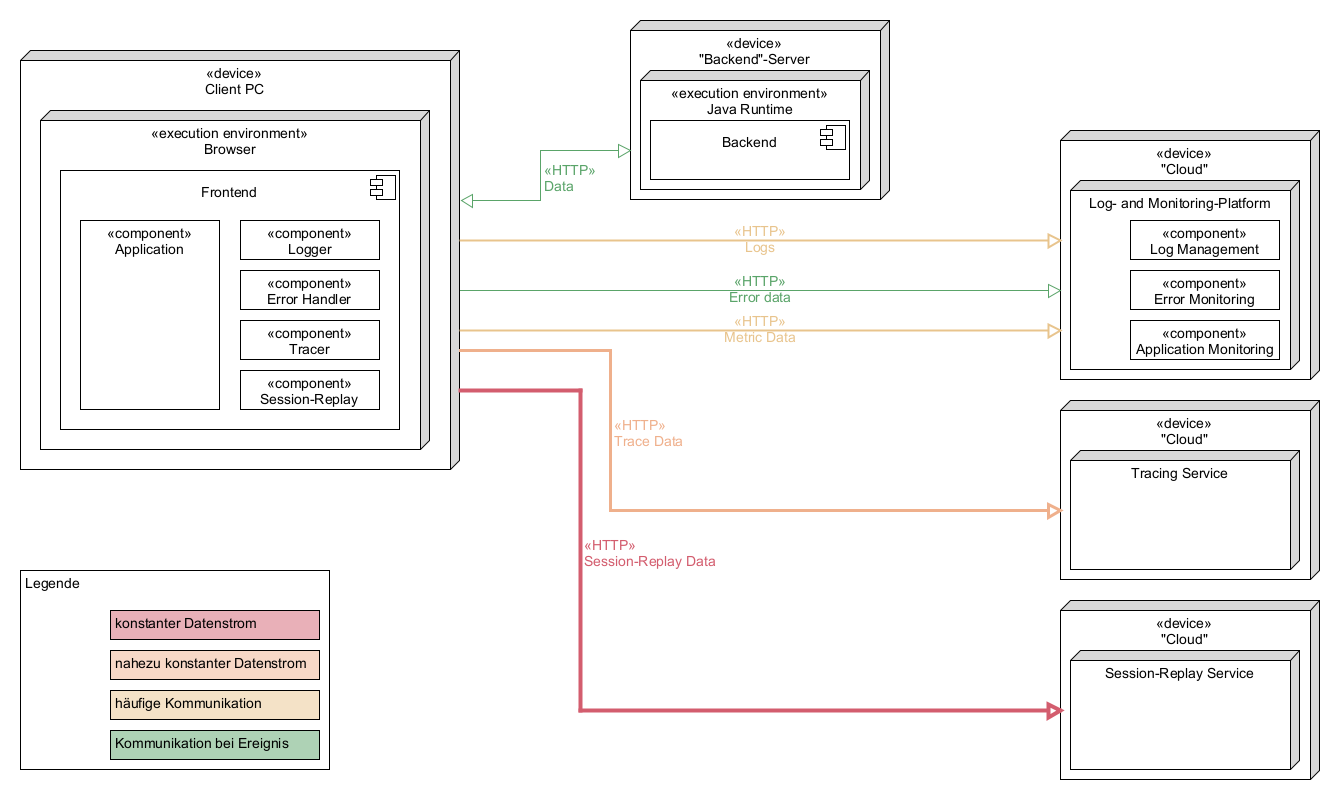
\includegraphics[width=0.75\linewidth]{img/04_erstellung-poc/konzept-datendurchsatz.png}
	\caption{Grobe Architektur mit hervorgehobenem Datendurchsatz}
	\label{fig:grobe-architektur-datendurchsatz}
\end{figure}

	\subsection{Technologie-Stack}
	\label{sec:technologie-stack}

	\textit{Welche Technologien werden eingesetzt, um die Architektur umzusetzen und zu erfüllen?}

	\subsection{Übertragbarkeit}

	\textit{Eignet sich das Konzept in Hinsicht auf Übertragbarkeit auf andere Softwareprojekte?}

	\textit{Dieser Punkt wird in Kapitel 5 erneut betrachtet und es wird versucht die tatsächliche Übertragbarkeit der erstellten Lösung zu erörtern.}

\section{Implementierung}

	\textit{Auf Basis des Konzeptes soll nun eine Implementierung erfolgen.}